\section{File server}

The file server is integrated with management interface, \emph{Central Management}, and allow us the configuration of main features of this service.

On \emph{ETFS} tab, we can access to the following interface.

\begin{figure}[H]
    \begin{center}
    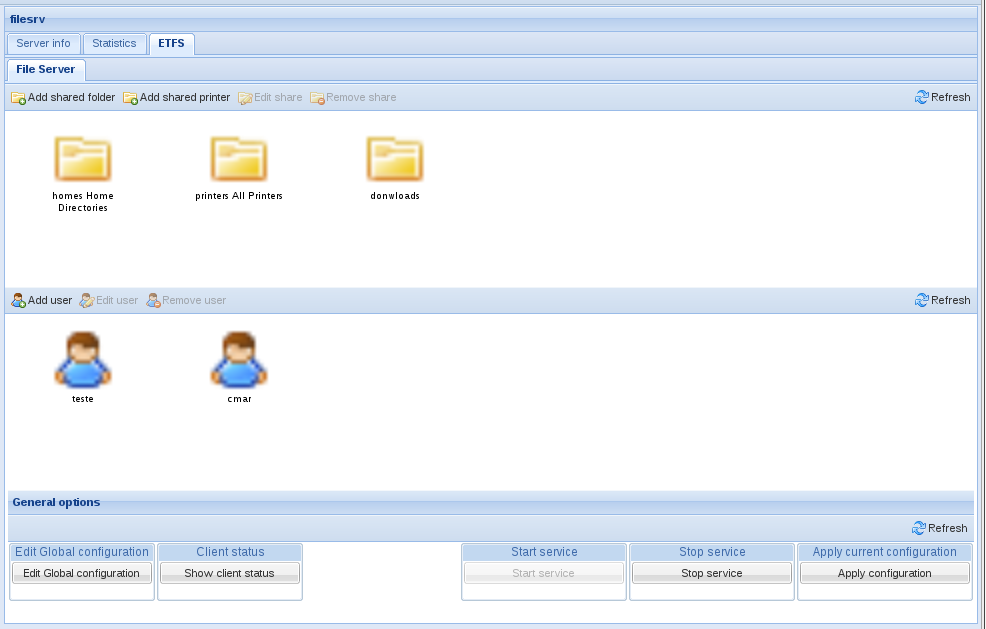
\includegraphics[scale=0.38]{screenshots/etfs/etfs_main.png}
    \caption{File server management interface}
    \label{fig:etfs_main}
    \end{center}
\end{figure}

On this interface we can do the management of all task of file server, such as, edit global configuration, start and stop the service, the management of shared folders, printers and users and get the status of user connections and of the file server service.

\begin{figure}[H]
    \begin{center}
    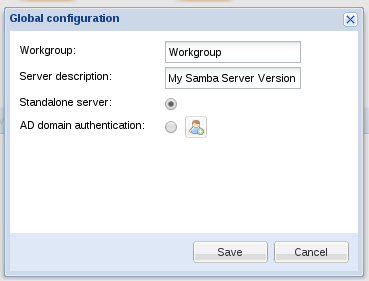
\includegraphics[scale=0.38]{screenshots/etfs/etfs_edit_global_config_user.png}
    \caption{Edit global configuration}
    \label{fig:etfs_global_config_user}
    \end{center}
\end{figure}

When edit global configuration we need to provides the \emph{workgroup}, optional, one description and the type of server configuration: standalone server or AD domain authentication.

On first case, the server use local authentication for the users and provides the management of them.

On second case, the server use authentication of domain and the users management has to be made on \emph{Active Directory}.

\begin{figure}[H]
    \begin{center}
    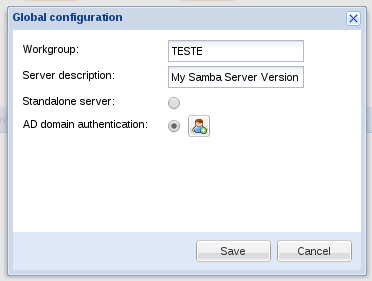
\includegraphics[scale=0.38]{screenshots/etfs/etfs_edit_global_config_ad.png}
    \caption{Edit global configuration with AD authentication}
    \label{fig:etfs_edit_global_config_ad}
    \end{center}
\end{figure}

For server configuration of \emph{Active Directory} domain authentication, it is required to join the server to the domain.
For do that, it is required to proceed to the configuration of domain, the server of \emph{Active Directory} and name and password of administrator of the domain as shown in figure \ref{fig:etfs_join_to_ad}.

\begin{figure}[H]
    \begin{center}
    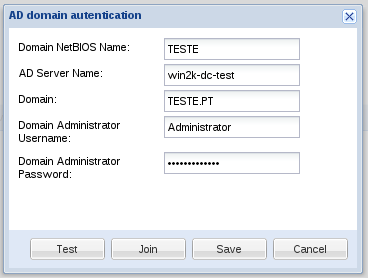
\includegraphics[scale=0.38]{screenshots/etfs/etfs_join_to_ad.png}
    \caption{Configuration of AD domain authentication}
    \label{fig:etfs_join_to_ad}
    \end{center}
\end{figure}

After configuration the global configuration of file server, we can proceed to the management of shared folders, printers and users.

\begin{figure}[H]
    \begin{center}
    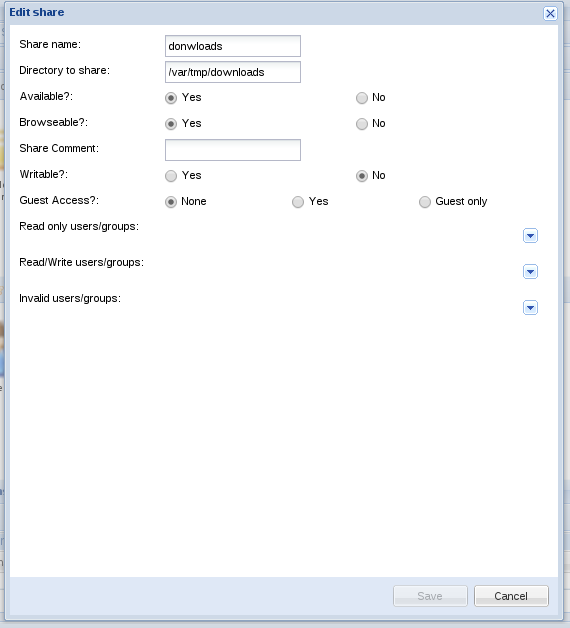
\includegraphics[scale=0.38]{screenshots/etfs/etfs_edit_file_share.png}
    \caption{Create/edit shared folder}
    \label{fig:etfs_edit_file_share}
    \end{center}
\end{figure}

\begin{figure}[H]
    \begin{center}
    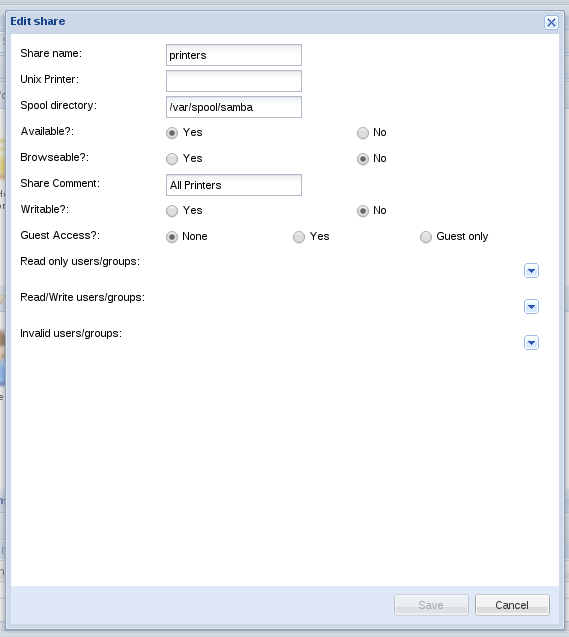
\includegraphics[scale=0.38]{screenshots/etfs/etfs_edit_printer_share.png}
    \caption{Create/edit shared printer}
    \label{fig:etfs_edit_printer_share}
    \end{center}
\end{figure}

\begin{figure}[H]
    \begin{center}
    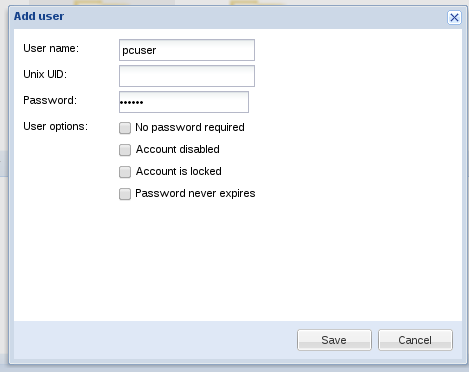
\includegraphics[scale=0.38]{screenshots/etfs/etfs_edit_user.png}
    \caption{Create/edit user}
    \label{fig:etfs_edit_user}
    \end{center}
\end{figure}

It is also possible to get information about status of users connections and the shared folder or service used for each one.

\begin{figure}[H]
    \begin{center}
    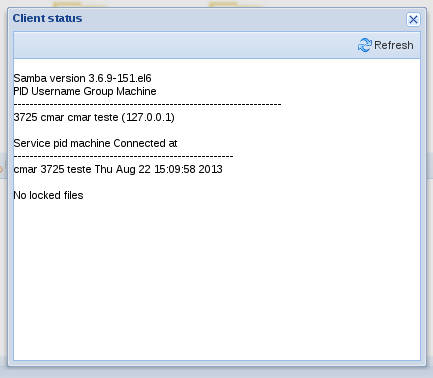
\includegraphics[scale=0.38]{screenshots/etfs/etfs_client_status.png}
    \caption{Information about status of users connections}
    \label{fig:etfs_client_status}
    \end{center}
\end{figure}

